\documentclass[11pt,a4paper]{article}
\usepackage[spanish,activeacute]{babel}
\usepackage[utf8]{inputenc}
\usepackage{amsmath}
\usepackage{amsfonts}
\usepackage{amssymb}
\usepackage{graphicx}
\usepackage{color}
\usepackage{listings}
\usepackage{amsthm}
\usepackage{caption}
\usepackage{subcaption}
\usepackage{dsfont}
\usepackage{comment}
\usepackage{enumerate}
\usepackage{mathtools,xparse}
\usepackage{ mathrsfs }
\usepackage{float}

\usepackage[left=2.10cm, right=2.10cm, top=2.50cm, bottom=2.50cm]{geometry}

\usepackage{tikz}
\usetikzlibrary{shapes,arrows}
\usetikzlibrary{babel}

\usepackage[]{hyperref}
\hypersetup{
    pdftitle={Informe EMV},
    pdfauthor={Mario Muñoz Mesa},
    pdfsubject={ },
    pdfkeywords={keyword1, keyword2},
    bookmarksnumbered=true,     
    bookmarksopen=true,         
    bookmarksopenlevel=1,       
    colorlinks=true,   
    linkcolor=black,         
    pdfstartview=Fit,           
    pdfpagemode=UseOutlines,
    pdfpagelayout=TwoPageRight
}


\title{\huge \bf Informe DB\_3.}
\author{Mario Muñoz Mesa}
\date{\today}

\begin{document}

	\maketitle
	\renewcommand*\contentsname{Índice}	
	\tableofcontents
	
	\newpage
    \section{Resumen.}
    Se tiene dataset consituido por observaciones de 11 variables en 34 estados del mundo.
    
    Tras recodificaciones, sobre cada variable se realiza: tratamiento de valores perdidos, análisis numérico clásico, tratamiento de outliers y análisis de normalidad.
    
    Con el objetivo de reducir la dimensión se ha aplicado Análisis de Componentes Principales (ACP) y Análisis Factorial (AF) donde se buscan factores ocultos. También se ha aplicado Clustering no jerárquico, k-means, para encontrar grupos de paises similares.
    
    La reducción de dimensionalidad tanto por ACP como AF es factible y se obtienen indicaciones de la mejor reducción por distintos métodos. En Clustering se observa buena agrupación en 2 grupos.

    \section{Introducción.}
    El dataset DB\_3 recoge observaciones de 11 variables en 34 estados del mundo. 
    
    En primer lugar se han corregido los nombres de algunos paises en el dataset. Se encuentra solo un valor perdido, y se imputan por la media del resto de instancias. Se analizan las distribuciones, con variedad de métricas asociadas, de cada variable en el análisis descriptivo numérico clásico. Los outliers encontrados en cada variable se corrigen sutituyéndolos por la media. También comprueba si existe normalidad en cada una de las variables. 
    
    Previo a las técnicas de reducción de dimensionalidad se comprueba correlación entre las variables. La regla de Abdi et al. (2010) es aplicada en ACP obteniendo 3 componentes principales con varianza explicada acumulada 0.80568. Se muestran gráficas comparativas de estas 3 componentes principales que muestran el peso de las variables en las componentes, así como gráficas que comparan el peso de cada instancia en cada componente principal, y gráficas combinando tanto peso de instancias como de variables en cada componente principal. En AF se busca número óptimo de factores por método Scree plot y Análisis Paralelo, al no ser suficientes se eligen 3 factores (1 más que el número óptimo). Se analizan, mostrando gráficas, la asociación de variables a cada factor.
    
    Se obtiene discrepancia sobre normalidad multivariante en test de Royston y Henze-Zirkler.
    
    En clustering, el Método del Codo (``within sum-of-squares'') y Método de Silhouette (``average silhouette width'') nos sugieren elegir 2 clusters. Se muestran gráficamente los clusters con las instancias de  cada uno, también se obtienen los valores medios de las variables en cada cluster.
    
    El objetivo ha sido encontrar información relevante univariante y multivariante, así como posibles reducciones de dimensionalidad con AF y ACP, y grupos similares.

	
	
    \section{Materiales y Métodos.}
    \subsection{Materiales.}
    Las variables del dataset son:
    \begin{itemize}
\item Ztlibrop: Número de libros publicados.
\item Ztejerci: Cociente entre el número de individuos en ejército de tierra y población total del
estado.
\item Ztpobact: Cociente entre población activa y total.
\item Ztenergi: Tasa de consumo energético.
\item Zpservi: Población del sector servicios.
\item Zpagricu: Población del sector agrícola.
\item Ztmedico: Tasa de médicos por habitante.
\item Zespvida: Esperanza de vida.
\item Ztminfan: Tasa de mortalidad infantil.
\item Zpobdens: Densidad de población
\item Zpoburb: Porcentaje de población urbana.
	\end{itemize}
	
	Mostramos tabla resumen de las variables, incluyendo la media y desviación típica. Ésta se obtiene ignorando el valor perdido en Ztlibrop:
	
	\begin{table}[H]
	\begin{center}
	\begin{tabular}{|c|c|c|c|c|c|c|c|}
	\hline
	  Variable & Media & Mediana & Desv. típica & Max & Min & 3rd Qu & 1st Qu \\
	\hline \hline
	ZPOBDENS & 0 & -0.1616 & 1	& 2.8616 & -1.0778	& 0.5547	&-0.8497 \\ \hline
	ZTMINFAN & 0 & -0.3931 & 1	& 1.9048 & -1.1026	&0.8985		&-0.9586 \\ \hline
	ZESPVIDA & 0 & 0.2781 & 1	& 1.2486 & -2.1453	&0.9033		&-0.7460 \\ \hline
	ZPOBURB & 0 & 0.1268 & 1	& 1.5096 & -1.7697	&0.8148		&-0.7320 \\ \hline
	ZTMEDICO & 0 & -0.2916 & 1	& 2.3717 & -1.1473	&0.8694		&-0.8829 \\ \hline
	ZPAGRICU & 0 & -0.2134 & 1	& 1.9052 & -1.2342	&0.7115	&-0.8480 \\ \hline
	ZPSERVI & 0 & 0.03541 & 1	& 1.62885 & -1.88521	&0.85176	&-0.72858 \\ \hline
	ZTLIBROP & 0 & -0.3237 & 1	& 2.4024 & -0.9696	&0.7736	&-0.9240 \\ \hline
	ZTEJERCI & 0 & 0.20626 & 1	& 4.42620 & -0.86586	&0.07996	&-0.59889 \\ \hline
	ZTPOBACT & 0 & -0.1067 & 1	& 1.7045 & -2.1341	&0.8789	&-0.6735 \\ \hline
	ZTENERGI & 0 & -0.3900 & 1	& 2.7498 & -0.9507	&0.5828	&-0.7813 \\ \hline

	\end{tabular}
	\caption{Tabla resumen de las variables.}
	\label{tabla:sencilla}
	\end{center}
	\end{table}
	
	\subsection{Métodos.}
	En el análisis numérico clásico, se visualizan los datos mediante Boxplot (\texttt{boxplot}), y se analiza: (1) media y medidas de centralidad resistentes: PMC, Trimedia y Centrimedia \iffalse (\texttt{PMC}, \texttt{Trimedia}, \texttt{Centrimedia})\fi, (2) desviación típica (\texttt{sd}), coef. variación (\texttt{sd}/\texttt{mean}), rango (\texttt{range}) y medidas resistentes (\texttt{Rang. Inter-Cuartílico}, \texttt{MEDA}, \texttt{CVc}), (3) medidas de forma como asimetría (\texttt{skewness}), curtosis (\texttt{kurtosis}), y medidas resistentes como Asimetría de Yule, Asimetría de Kelly y Asimetría de Kelly adimensional.
	
	Para el análisis de la normalidad de cada variable se ha empleado gráfico Q-Q (\texttt{qqnorm}). Se comprueba que hay correlaciones significativas en las variables empleando el test de esfericidad de Bartlett (\texttt{cortest.bartlett}), también se visualizan estas correlaciones (\texttt{ggcorrplot}). 
	
	Se aplica Análisis de Componentes Principales (\texttt{prcomp}), analizando las varianzas explicadas individuales y acumuladas. Para selección de componentes se emplea la regla de Abdi et al. (2010). Se analizan pesos de variables en cada componente (\texttt{fviz\_pca\_var}), de instancias en cada componente (\texttt{fviz\_pca\_ind}), y de variables e instancias en cada componente (\texttt{fviz\_pca}).

	En el empleo de Análisis Factorial se busca el número óptimo de factores por método Scree plot (Cattel 1966) (\texttt{scree}) y Análisis Paralelo (Horn 1965) (\texttt{fa.parallel}). Se emplean rotaciones varimax buscando mayor interpretabilidad, mostrando diagrama (\texttt{fa} y \texttt{fa.diagram} respect.). También se contrasta si el número de factores es suficiente (\texttt{factanal}).
	
	Los test de Royston y Henze-Zirkler son los empleados para analizar la normalidad multivariante (\texttt{royston\_test} y \texttt{mvn(...,mvnTest=``hz'')} respectivamente).
	
	Para Análisis Cluster se muestra matriz de distancias (\texttt{fviz\_dist}) y se emplea k-means (\texttt{kmeans}), dibujando gráficamente los clusters (\texttt{fviz\_cluster}). La búsqueda de número óptimo de clusters es realizada empleando métodos ``within sum of square'', ``average silhouette width'', ``gap statistics'', (\texttt{fviz\_nbclust}).
    \section{Resultados.}
    \subsection{Análisis exploratorio univariante.}
    Se encontró 1 valor perdido en ZTLIBROP, lo que supone un 2.94117647 \% de los datos, por lo que se imputa por la media. 
    
    \begin{figure}[H]
		\centering
		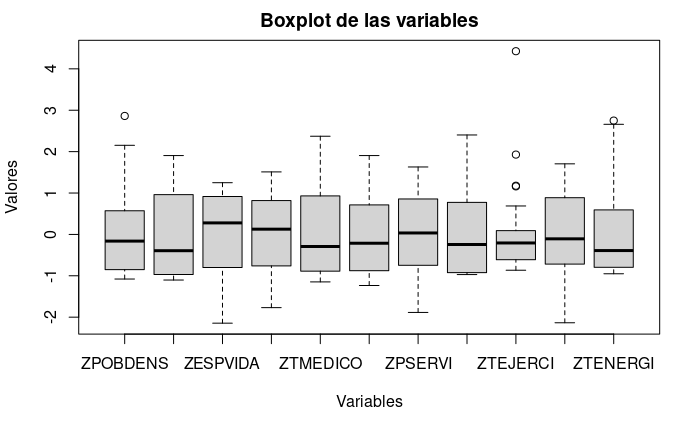
\includegraphics[width=0.8\textwidth]{images/boxplot_uni}
		\caption{Boxplot de cada variable.}
	\end{figure}
	Observamos 1 outlier en ZPOBDENS y ZTENERGI, varios en ZTEJERCI. Los sustituimos por la media.
	
	Destacamos que
	\begin{itemize}
		\item ZTLIBROP presenta fuerte asimetría hacia la derecha, así como desplazamiento a la derecha y concentración de los datos por el alto valor de curtosis.
		\begin{figure}[H]
		\centering
		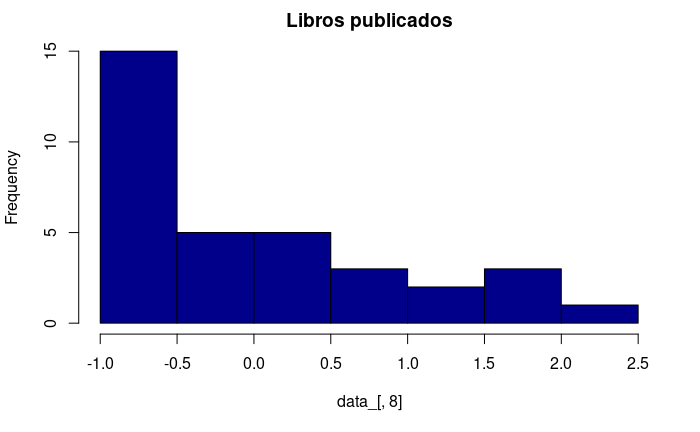
\includegraphics[width=0.55\textwidth]{images/ztlibrop}
		\caption{Distribución de ZTLIBROP.}
	\end{figure}
	
		\item ZTEJERCI también presenta muy fuerte asímetría a la derecha, desplazamiento de las medidas resistentes de centralidad a la izquierda, así como alta concentración de los datos por valor muy alto de curtosis.
		
		\begin{figure}[H]
		\centering
		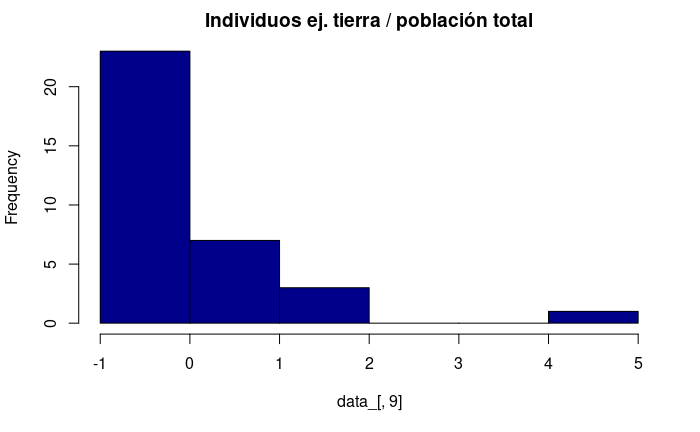
\includegraphics[width=0.55\textwidth]{images/ztejerci}
		\caption{Distribución de ZTEJERCI.}
	\end{figure}
	\end{itemize}
	
	
	
	Obtenemos gráficos Q-Q de las variables,
	\begin{figure}[H]
		\centering
		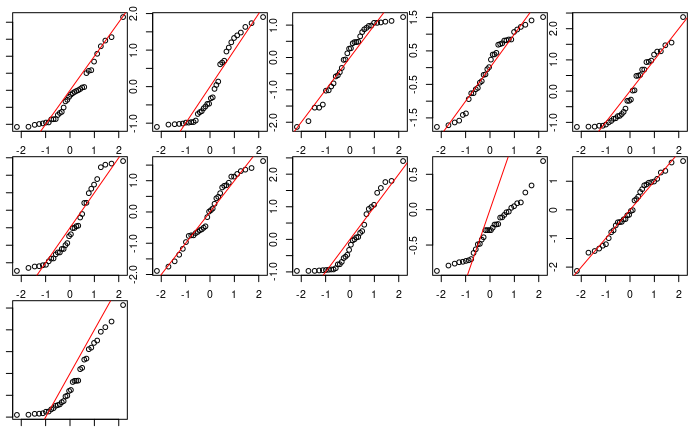
\includegraphics[width=0.8\textwidth]{images/qqplot}
		\caption{Gráficos Q-Q.}
	\end{figure}
	Vemos que las variables que más se acercan a la normalidad son la 4, 6, 7 y 10 (ZPOBURB, ZPAGRICU, ZPSERVI y ZTPOBACT), en menor medida la 1, 2, 3, 5, 8 y 11 (ZPOBDENS, ZTMINFAN, ZESPVIDA, ZTMEDICO, ZTLIBROP y ZTENERGI), la que menos se acerca a normalidad es la 9 (ZTEJERCI).
	
    \subsection{Análisis exploratorio multivariante.}
    Una vez con los datos normalizados, encontramos correlaciones entre las variables:
	\begin{figure}[H]
		\centering
  \subfloat[ggcorrplot]{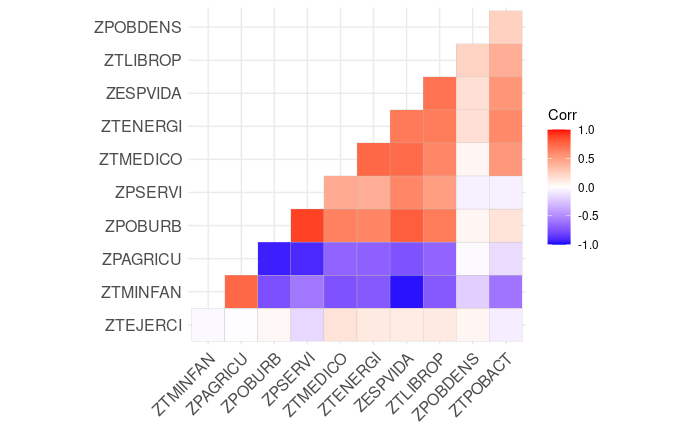
\includegraphics[width=0.4\textwidth]{images/matriz_corr2}\label{fig:f1}}
  \hfill
  \subfloat[rplot]{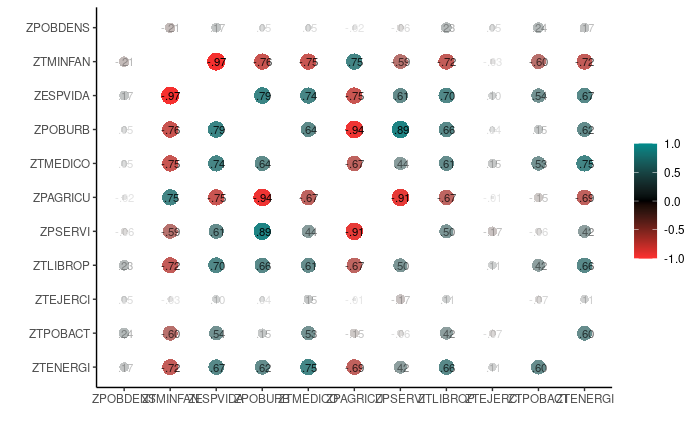
\includegraphics[width=0.6\textwidth]{images/matriz_corr}\label{fig:f2}}
	\end{figure}
	El test de esfericidad de Bartlett arroja p-valor 1.583951e-51, se rechaza hipótesis nula por lo que las correlaciones son significativamente distintas de 0.
	
	Tiene por tanto sentido el Análisis de Componentes Principales y Análisis Factorial.
    \subsubsection{Análisis de Componentes Principales.}
    Mostramos gráficamente las varianzas explicadas de cada componente principal:
    \begin{figure}[H]
		\centering
		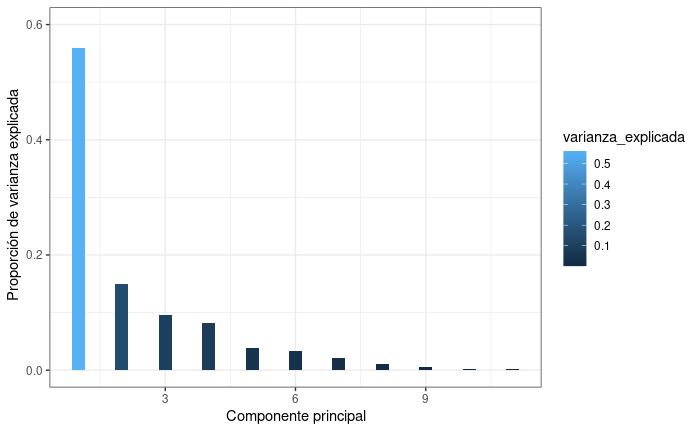
\includegraphics[width=0.7\textwidth]{images/var_exp}
		\caption{Proporción de varianza explicada de cada componente principal.}
	\end{figure}
	y la proporción de varianza acumulada:
	\begin{figure}[H]
		\centering
		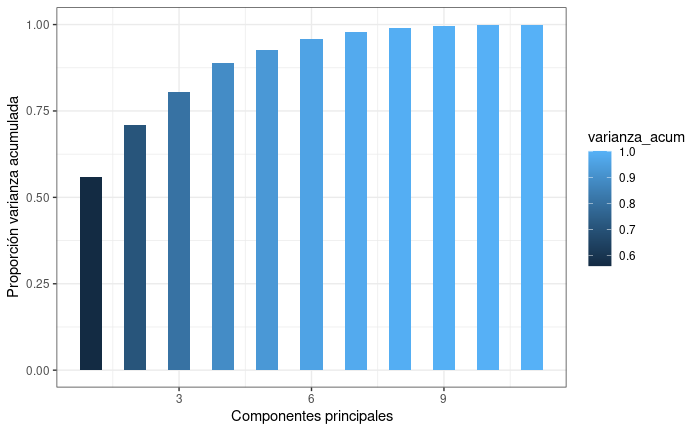
\includegraphics[width=0.7\textwidth]{images/var_exp_acum}
		\caption{Proporción de varianza explicada de cada componente principal.}
	\end{figure}
	
	Para la selección de componentes principales utilizamos la regla de Abdi et al. (2010), y nos quedamos con las tres primeras componentes principales pues tienen proporción de varianza explicada superior a 1, que es la media. Estas 3 componentes principales nos dan varianza explicada acumulada 0.80568.
	
	Visualizamos el peso de cada variable en las componentes principales, junto con la contribución de cada individuo de la muestra.
	
	\begin{itemize}
	\item Primera y segunda componentes principales:	
	\begin{figure}[H]
		\centering
		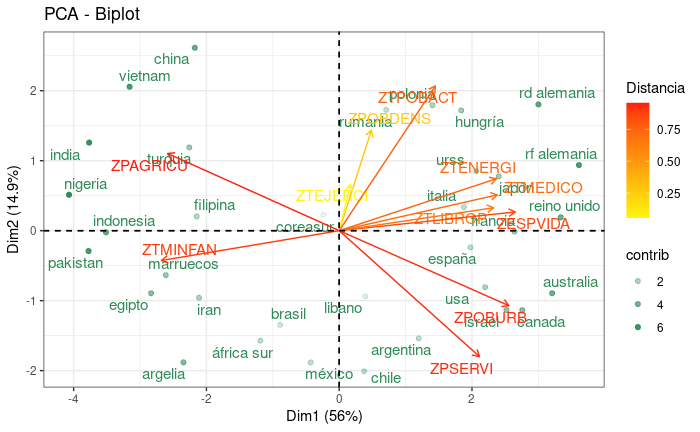
\includegraphics[width=0.7\textwidth]{images/vis_pca1}
		\caption{Pesos de variables e individuos en las componentes principales.}
	\end{figure}
	\item Primera y tercera componentes principales:
	\begin{figure}[H]
		\centering
		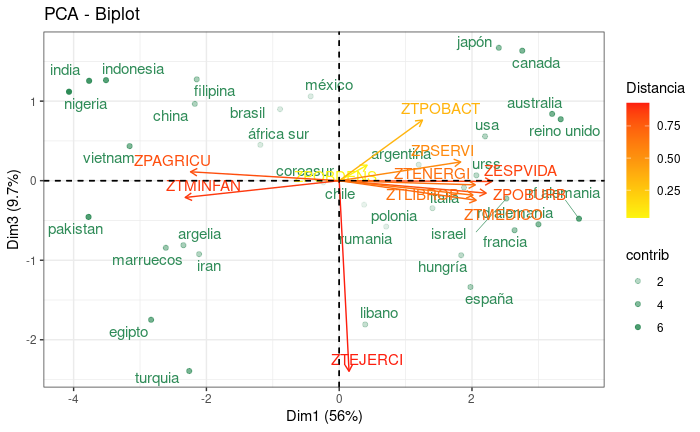
\includegraphics[width=0.7\textwidth]{images/vis_pca2}
		\caption{Pesos de variables e individuos en las componentes principales.}
	\end{figure}
	\item Segunda y tercera componentes principales:
	\begin{figure}[H]
		\centering
		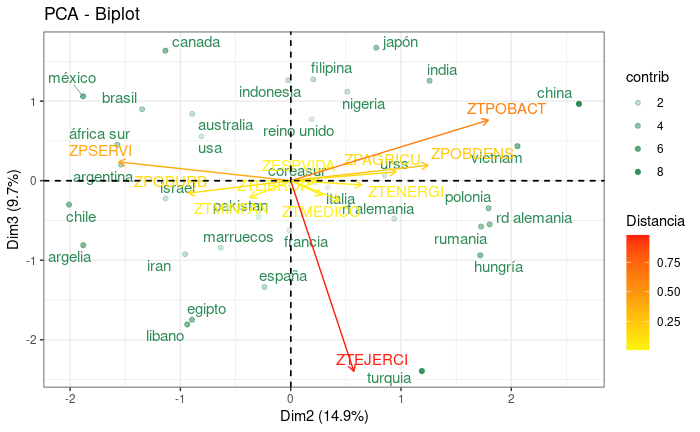
\includegraphics[width=0.7\textwidth]{images/vis_pca3}
		\caption{Pesos de variables e individuos en las componentes principales.}
	\end{figure}
	\end{itemize}
	
	Analizando las 3 gráficas observamos que:
	\begin{itemize}
		\item En la primera componente principal tienen mayor peso variables como APAGRICU, ATMINFAN, ZESPVIDA y ZTMEDICO, e instancias (paises) como india, nigeria, pakistán, alemania, reino unido y australia.
		\item En la segunda componente principal tienen mayor peso variables como ZTPOBACT, ZPOBDENS y ZPSERVI, e instancias (paises) como china, argelia, méxico y chile.
		\item En la tercera componente principal destaca con gran peso la variable ZTEJERCI, e instancias (paises) como canada, japón y turquía.
	\end{itemize}
    \subsubsection{Análisis Factorial.}
    Determinaremos el número óptimo de factores por método Scree plot (Cattel 1966) y Análisis Paralelo (Horn 1965):
    \begin{figure}[H]
		\centering
  \subfloat[Scree plot]{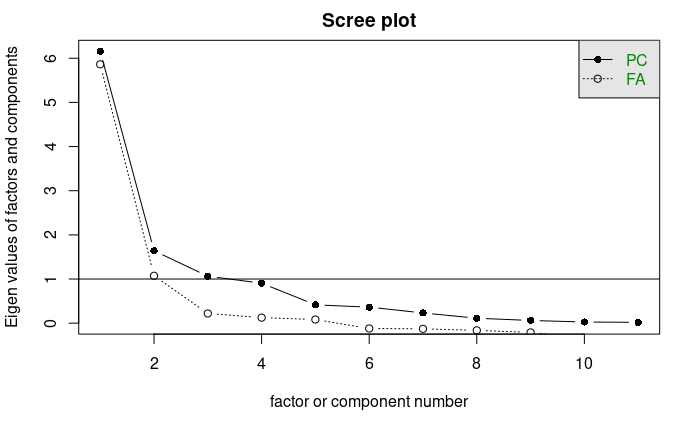
\includegraphics[width=0.5\textwidth]{images/scree}\label{fig:f1}}
  \hfill
  \subfloat[Parallel analysis]{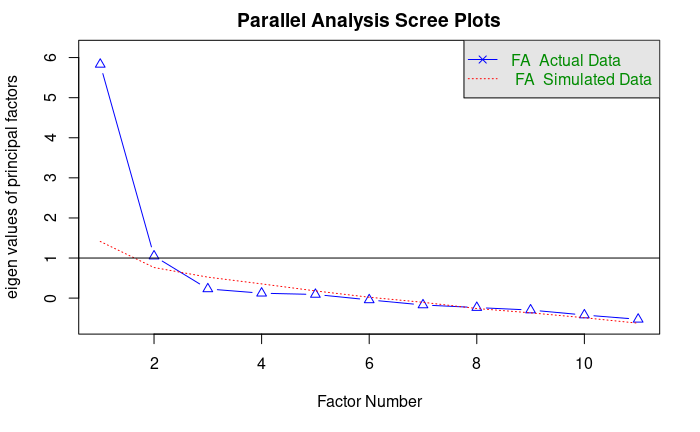
\includegraphics[width=0.5\textwidth]{images/scree_parallel}\label{fig:f2}}
  \caption{Gráficos de Scree plot y Análisis Paralelo}
	\end{figure}
	
	El Análisis Paralelo nos sugiere 2 factores, sin embargo al contrastar con test de hipótesis si 2 factores son suficientes se obtiene p valor 0.00176, 2 no son suficientes. Por lo que se toman 3 factores que nos arroja p-valor 0.397 y por tanto no se rechaza la hipótesis nula.\\
	
	Encontramos interpretabilidad tras realizar rotación varimax:
	\begin{figure}[H]
		\centering
		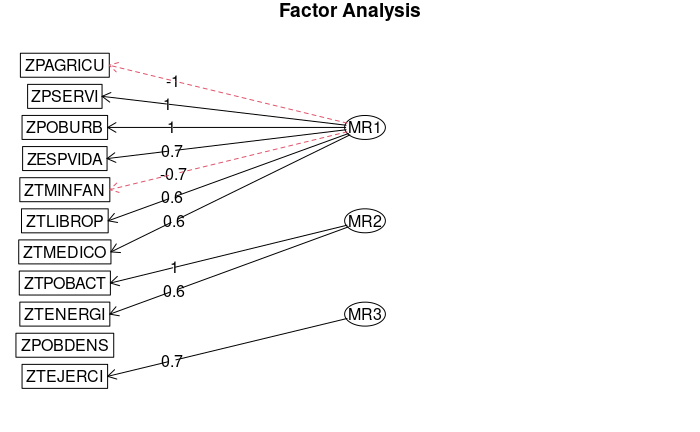
\includegraphics[width=0.7\textwidth]{images/inter_fa}
		\caption{Asociaciones de variables con los factores.}
	\end{figure}
	
	Vemos que el primer factor está asociado con ZPAGRICU, ZPOBURB,ZPSERVI, ZESPVIDA, ZTMINFAN, ZTLIBROP y ZTMEDICO, mientras que el segundo factor está asociado con ZTPOBACT y ZTENERGI, el tercero con ZTEJERCI.
	\subsubsection{Análisis de la normalidad multivariante.}
	Encontramos 11 outliers 
	\begin{figure}[H]
		\centering
		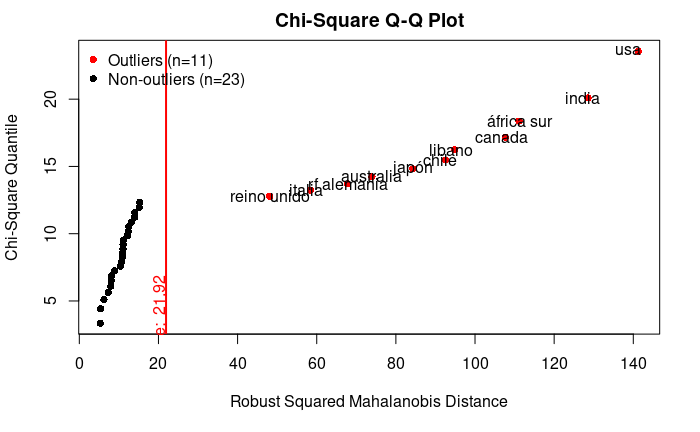
\includegraphics[width=0.7\textwidth]{images/out_mult}
		\caption{Chi-Square Q-Q Plot.}
	\end{figure}
	
	El test de Royston nos da p-valor 7.374655e-05, indica rechazar la hipótesis nula, no tendríamos normalidad multivariante. El test de Henze-Zirkler da p-valor 0.0761232, no rechazamos la hipótesis nula de normalidad multivariante. No encontramos suficiente evidencia de normalidad multivariante.
    \subsubsection{Clustering.}
    En la matriz de distancias se intuyen 2 agrupaciones:
    \begin{figure}[H]
		\centering
		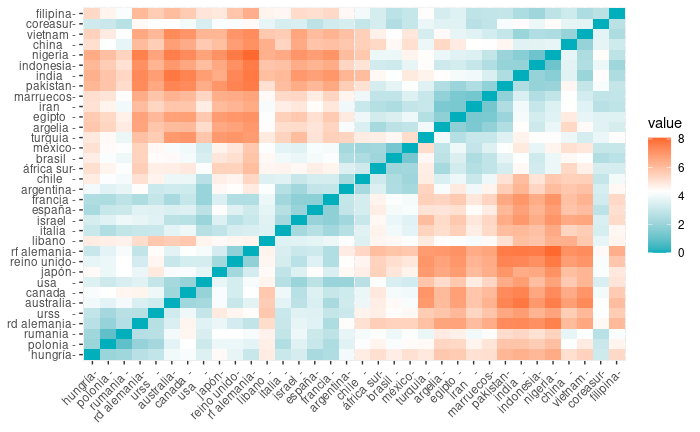
\includegraphics[width=0.7\textwidth]{images/dist_matrix}
		\caption{Matriz de distancias.}
	\end{figure}
	
	Buscamos el número óptimo de clusters, para ello se aplicamos Método del Codo (``within sum-of-squares''), Método de Silhouette (``average silhouette width'') y Método estadístico de brecha (GAP) (``gap statistics'').
	
	\begin{figure}[H]
		\centering
		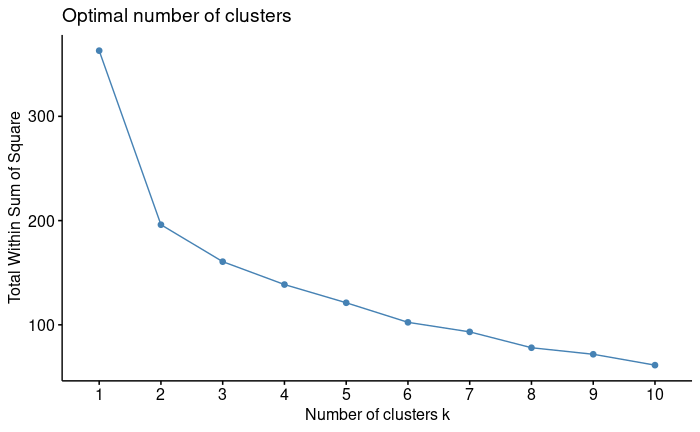
\includegraphics[width=0.55\textwidth]{images/wss}
		\caption{within sum-of-squares}
	\end{figure}
	
	\begin{figure}[H]
		\centering
		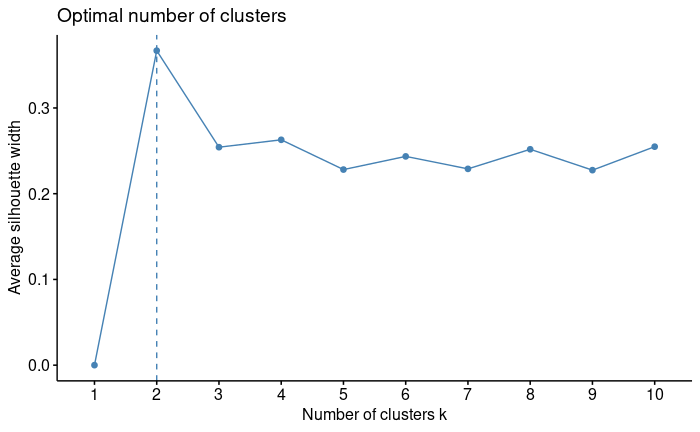
\includegraphics[width=0.55\textwidth]{images/silhouette}
		\caption{average silhouette width}
	\end{figure}
	
	\begin{figure}[H]
		\centering
		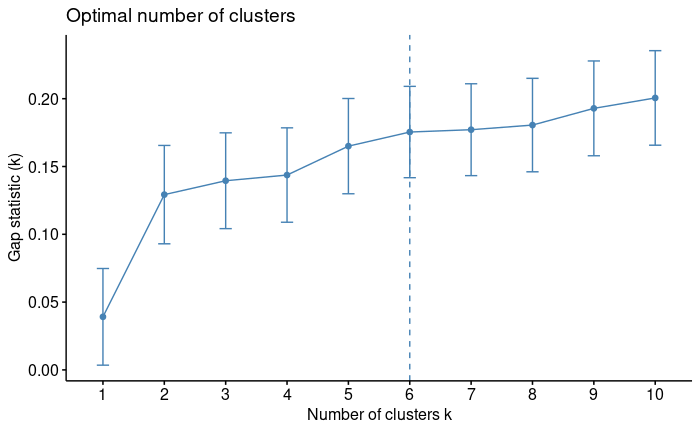
\includegraphics[width=0.55\textwidth]{images/gap}
		\caption{gap statistics}
	\end{figure}
	
	Tanto ``within sum-of-squares'' como ``average silhouette width'' no sugieren $K=2$ como número de clusters más adecuado.
	
	La agrupación quedaría:
	\begin{figure}[H]
		\centering
		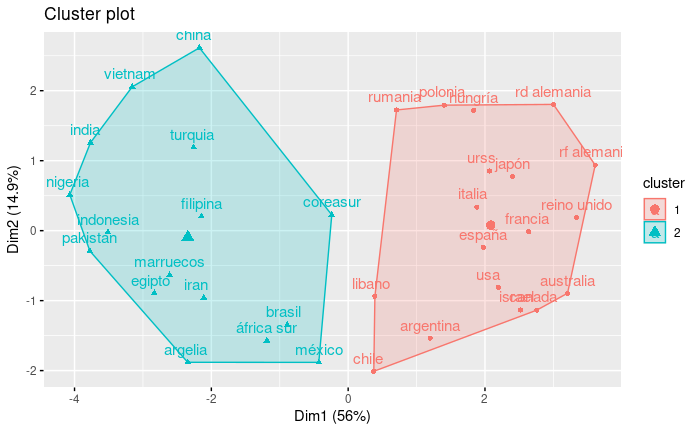
\includegraphics[width=0.7\textwidth]{images/2clusters}
		\caption{Los 2 clusters encontrados.}
	\end{figure}
	
	Se obtiene en un mismo grupo a: China, Vietnam, India, Nigeria, Indonesia, Pakistán, Turquía, Finipinas, Corea del Sur, Marruecos, Egipto, Irán, Brasil, África del Sur, Argelia y México; el resto de países en el otro grupo.
	
	Finalmente, mostramos medias de las variables a nivel de cluster:
	
	\begin{table}[H]
	\begin{center}
	\resizebox{17.4cm}{!} {
	\begin{tabular}{|c|c|c|c|c|c|c|c|c|c|c|c|}
	\hline
	  Cluster & ZPOBDENS & ZTMINFAN & ZESPVIDA & ZPOBURB & ZTMEDICO & ZPAGRICU & ZPSERVI & ZTLIBROP & ZTEJERCI  & ZTPOBACT & ZTENERGI\\
	\hline \hline
	1 & 0.2043031 & -0.7853941 & 0.7769316 & 0.7240592 & 0.7671309 & -0.7448802 & 0.5956415 & 0.6366902 & 0.1499519 & 0.4474332 & 0.6725565 \\ \hline
	2 & -0.2298410 & 0.8835684	 & -0.8740481 & -0.8145666	 & -0.8630222	 & 0.8379902	 & -0.6700966 & -0.7162765 & -0.1686959 & -0.5033623 & -0.7566261 \\ \hline
	\end{tabular}
	}
	\caption{Medias de las variables a nivel de cluster.}
	\label{tabla:sencilla}
	\end{center}
	\end{table}
	\section{Discusión.}
	Búscabamos información univariante relevante, los datos estaban efectivamente normalizados pero encontramos 1 valor perdido en ZTLIBROP, y outliers en ZPOBDENS, ZTEJERCI, ZTENERGI. No todas las variables sugieren seguir una normal, en especial ZTEJERCI es la que menos.
	
	Búscabamos información multivariante, donde hemos comprobado por test de esfericidad de Bartlett que los datos no están incorrelados. Esto nos permite aplicar ACP y AF. 
	
	En ACP, por la regla Abdi et al. (2010), seleccionamos las 3 primeras componentes principales, que nos dieron varianza explicada acumulada 0.80568. También hemos obtenido gráficas con los pesos de variables e individuos (paises) en cada componente principal, y las hemos analizado.
	
	En AF, 2 factores eran los óptimos según método Scree plot y Análisis paralelo, sin embargo en contraste de hipótesis observamos que 2 no son suficientes. Se toman 3 factores que ya sí eran suficientes, donde el primer factor está asociado con ZPAGRICU, ZPOBURB, ZPSERVI, ZESPVIDA, ZTMINFAN, ZTLIBROP y ZTMEDICO, el segundo factor está asociado con ZTPOBACT y ZTENERGI, el tercero con ZTEJERCI.
	
	En Clustering ya podían intuirse 2 grupos en la matriz de distancias. Se buscó el número óptimo por distintos métodos. Total Within Sum of Square y Average Silhouette width nos sugerían 2 clusters. Se obtuvieron 2 clusters de tamaño similar, 16 instancias en uno y 18 en el otro, y con coef. Silhouette elevado.
	\section{Conclusión.}
	No se encuentra suficiente evidencia de normalidad multivariante. Se observa correlación entre las variables. Se obtuvieron 3 componentes principales con varianza explicada acumulada considerable. Los 3 factores obtenidos en AF no fueron los óptimos. Obtuvimos 2 clusters diferenciados.
	
	Sin embargo, en el desarrollo se tuvo que imputar un valor perdido en una de las variables, así como se sustituyeron outliers presentes en otras variables.\\
	
	 Por otra parte, también estamos limitados a las variables e instancias proporcionadas, mayor cantidad de instancias y variables podrían proporcionarnos grupos de mayor calidad (más diferenciados) en Clustering.
	
	Otros caminos que podrían seguirse en Clustering son: (1) realizar Clustering tras reducción de dimensionalidad con ACP por ejemplo, (2) realizar Clustering mediante método jerárquico.
    

\end{document}
